\documentclass{standalone}
\usepackage{pgfplots}
\pgfplotsset{compat=1.17}

\colorlet{green_set}{green!70!black}
\colorlet{purple_set}{blue!80!cyan!60!red!95!black!90}
\colorlet{red_set}{red!80!black}

\begin{document}
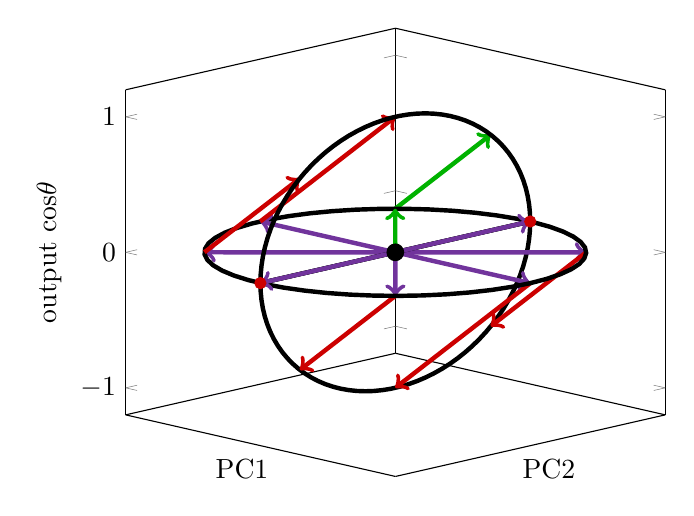
\begin{tikzpicture}
    \begin{axis}[
      view={45}{15},
      xtick=\empty,
      xlabel={PC1},
      ytick=\empty,
      ylabel={PC2},
      zlabel={output cos$\theta$},
    ]

    % Draw the ring in the x=0 plane
    \addplot3 [
      samples=50,
      domain=pi:2*pi,
      no marks,
      ultra thick,
    ] (0, {cos(deg(x))}, {sin(deg(x))});

    % Draw arrow from origin to 45 degree point on z=0 plane
    \draw[->, ultra thick, green_set] (axis cs:{cos(135)},{sin(135)},0) -- (axis cs:0,{sin(135)},{sin(135)});

    \draw[->, ultra thick, purple_set] (axis cs:0,0,0) -- (axis cs:{cos(45)},{sin(45)},0);
    \draw[->, ultra thick, red_set] (axis cs:{cos(45)},{sin(45)},0) -- (axis cs:0,{sin(45)},{-sin(45)});

    \draw[->, ultra thick, purple_set] (axis cs:0,0,0) -- (axis cs:{cos(0)},{sin(0)},0);
    \draw[->, ultra thick, red_set] (axis cs:{cos(0)},{sin(0)},0) -- (axis cs:0,{sin(0)},-1);

    \draw[->, ultra thick, purple_set] (axis cs:0,0,0) -- (axis cs:{cos(-45)},{sin(-45)},0);
    \draw[->, ultra thick, red_set] (axis cs:{cos(-45)},{sin(-45)},0) -- (axis cs:0,{sin(-45)},{sin(-45)});

    \draw[->, ultra thick, purple_set] (axis cs:0,0,0) -- (axis cs:{cos(-135)},{sin(-135)},0);

    % Draw the ring in the z=0 plane
    \addplot3 [
      samples=50,
      domain=0:2*pi,
      no marks,
      ultra thick,
    ] ({cos(deg(x))}, {sin(deg(x))}, 0);

    \draw[->, ultra thick, green_set] (axis cs:0,0,0) -- (axis cs:{cos(135)},{sin(135)},0);

    \draw[->, ultra thick, red_set] (axis cs:{cos(-135)},{sin(-135)},0) -- (axis cs:0,{sin(-135)},{-sin(-135)});
    
    \draw[->, ultra thick, purple_set] (axis cs:0,0,0) -- (axis cs:{cos(180)},{sin(180)},0);
    \draw[->, ultra thick, red_set] (axis cs:{cos(180)},{sin(180)},0) -- (axis cs:0,{sin(180)},{1});

    % Draw the ring in the x=0 plane
    \addplot3 [
      samples=50,
      domain=0:pi,
      no marks,
      ultra thick,
    ] (0, {cos(deg(x))}, {sin(deg(x))});

    \draw[->, ultra thick, purple_set] (axis cs:0,0,0) -- (axis cs:{cos(90)},{sin(90)},0);

    \draw[->, ultra thick, purple_set] (axis cs:0,0,0) -- (axis cs:{cos(90)},{-sin(90)},0);

    \filldraw[red_set] (axis cs:{cos(90)},{sin(90)},0) circle (2pt);
    \filldraw[red_set] (axis cs:{cos(90)},{-sin(90)},0) circle (2pt);
    \filldraw (axis cs:0,0,0) circle (3pt);
    
    \end{axis}
\end{tikzpicture}
\end{document}